\chapter{The \texorpdfstring{$P(3, -3, n)$}{P(3, -3, n)} family}\label{ch:pretzel}
\section{Motivation}\label{sec:motivation}
There is no general method of finding Lagrangian cobordisms, and there are very few sufficient conditions for their existence.
A natural way of refining this question is to restrict either $K_-$ or $K_+$.
In particular, we want to know under what conditions there exists a decomposable cobordism from the unknot $U$ to some Legendrian knot $K$. This choice is not arbitrary: it is unclear whether any of the known obstructions give information about the existence of such cobordisms when $\maxtb K \leq -1$.

A good candidate for this search is the class of knots called ribbon knots, which we define here.

\begin{definition}
    A knot $K$ is said to be \textbf{ribbon} if $K$ bounds a smoothly embedded disk $d: D \to \R^3$ with only ribbon singularities.
    That is, every region of self-intersection of $d$ is an arc $A \in \R^3$ such that the preimage of $A$, $d^{-1} (A)$, consists of two arcs in $D$ of which one is within the interior of $D$ and the other has its endpoints on the boundary of $D$.
\end{definition}

This definition is more clear alongside a ribbon diagram, Figure~\ref{fig:ribbon-knots}.

\begin{figure}[ht!]
    \centering
    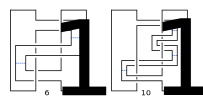
\includegraphics[width=0.8\linewidth]{images/ribbons.pdf}
    \caption{Diagrams for some ribbon knots, with the arcs of self-intersection marked in blue. The forms of these ribbons come from \cite{kawauchi}.}
    \label{fig:ribbons}
\end{figure}

Ribbon knots are a natural class to try to find Lagrangian cobordisms to, as topologically there always exist smooth cobordisms between the unknot and any ribbon knot.
In the case of Legendrian knots, it is known that ribbon knots admit decomposable Lagrangian cobordisms from sufficiently stabilized unknots \cite{leverson-etnyre}.
In the example of a ribbon knot with one band, we start from an untwisted unknot, add a second unknot with a zero-handle, and then use Legendrian isotopy to "pass" the tip of the first unknot through the two loops as desired, before finally using a 1-handle to join the ribbon tip to the second unknot, thus closing the knot. 

The cobordism created by these moves is necessarily a concordance: Each 1-handle adds a separate component to the link, and the 0-handle only adds genus if between two cusps of the same component.
Thus to construct such a cobordism to a Legendrian ribbon knot $K$, we have to start with a Legendrian unknot $U$ with $\tb U = \tb K$. Given the topological knot type of $K$, the unknot and $K$ must certainly have $\tb \leq \maxtb K$.
It is an open question when this can be achieved with equality: that is, when a cobordism can be constructed from a stabilized unknot to a maximal $\tb$-Legendrian ribbon knot.

\section{Constructions of Cobordisms}\label{sec:thm-a-proof}
The main result of this project, Theorem~\ref{thm:mine}, is the demonstration of an infinite family of knots, each of which has a maximal $\tb$-Legendrian representative admitting such a cobordism from the unknot.

\begin{mythm}\label{thm:mine}
    Let $P_n = P(3, -3, n)$, for $n$ an integer. Then there exists a Legendrian representative $K$ of $P_n$, and a Legendrian unknot $U$ with $\tb K = \tb U = \maxtb P_n$, such that there is a decomposable Lagrangian concordance from $U$ to $K$.
\end{mythm}

Figure~\ref{fig:pretzel-knot} shows a diagram of a knot in this family.
For example, $P(3, -3, 0) = 3_1 \# m(3_1)$. Further, $P_1 = 6_1$; $P_2 = 8_{20}$; $P_3 = 9_{46}$; and $P_4 = 10_{140}$. Further note that $P_n = m(P_{-n})$ \cite{kawauchi}.

\begin{figure}[ht!]
    \centering
    \includegraphics[width=0.4\textwidth]{images/pretzel-knot.pdf}
    \label{fig:pretzel-knot}
    \caption{The pretzel knot $P(3, -3, n)$. On the right, there are $n$ left half-twists if $n$ is positive, and $|n|$ \emph{right} half-twists if $n$ is negative.}
\end{figure}

We break the proof of this theorem into the following two lemmas.
\begin{lemma}\label{lem:tb}
    \[
        \maxtb P_n = \min \{ n-4, -1\}.
    \]
\end{lemma}

\begin{lemma}\label{lem:cobordism}
    For each $P_n$, there exists a Legendrian representative $K$ of $P_n$ and a stabilized Legendrian unknot $U$ such that 
    \[
        \tb K = \tb U = \min \{n-4, -1\},
    \]
    and there exists a decomposable Lagrangian concordance from $U$ to $K$.
\end{lemma}

The proof of Theorem~\ref{thm:mine} follows trivially from Lemmas~\ref{lem:tb}~and~\ref{lem:cobordism}, which we prove here.

\begin{proof}[Proof of Lemma~\ref{lem:tb}]

    We first compute the minimal degree of $a$ in the Kauffman polynomial of $P_n$; as this will give us a bound on $\maxtb P_n$ by Theorem~\ref{kauffman-bound}. We use the method from \cite{lu-zhong} for computing the Kauffman polynomial of a pretzel knot, and find that the minimal degree of $a$ in $Y(P_n)$ is given by $\min\{n-4, -1\}$. We implemented this computation in Mathematica; for details see Appendix~\ref{ch:appendix}.
    
    By Theorem~\ref{thm:ng} (Ng), the Kauffman bound is sharp for the pretzel link $P(3, -3, n)$ except when $n = 0$ or $n = \pm 2$. That is, $\maxtb P_n = \min\{n-4, -1\}$ for $n \neq 0$ and $n \neq \pm 2$. We will deal with these cases presently.

    In the case where $n = 0$, $P_0 = 3_1 \# m(3_1)$. The Thurston-Bennequin number of a connected sum is well known (\cite{torisu}, \cite{honda}). In particular,
    \[
        \maxtb{K_1 \# K_2} = \maxtb K_1 + \maxtb K_2 + 1.
    \]
    Thus $\maxtb P_0 = -6 + 1 + 1 = -4$ as desired.

    In the case where $n = \pm 2$, we have $P_2 = 8_{20}$ and $P_{-2} = m(8_{20})$, and therefore $\maxtb P_2 = -2 = 2-4$ and $\maxtb P_{-2} = -6 = -2-4$ as desired.

    Note that we have obtained the values for $\maxtb$ of $3_1$ and $8_{20}$ from \cite{atlas}.

\end{proof}


\begin{proof}[Proof of Lemma~\ref{lem:cobordism}]

    Depending on the value of $n$, there are five cases.

    In each, we first construct a suitable unknot $U$ with the desired $\tb$, using stabilizations and RI moves to add a total of $n-1$ half-twists, and we show the form of the desired Legendrian representative $K$. We then use the decomposable moves to describe a decomposable Lagrangian cobordism from $U$ to $K$. 

\begin{itemize}

    \item[$n \leq 0$ :]
        The desired $\tb$ is $n-4$. We start with an unknot as seen below, stabilized $|n - 1|$ times in order to add $|n - 1|$ left half-twists. Pictured here is $P_{-2}$, with 3 left half-twists.
        \begin{figure}[h!]
            \centering
            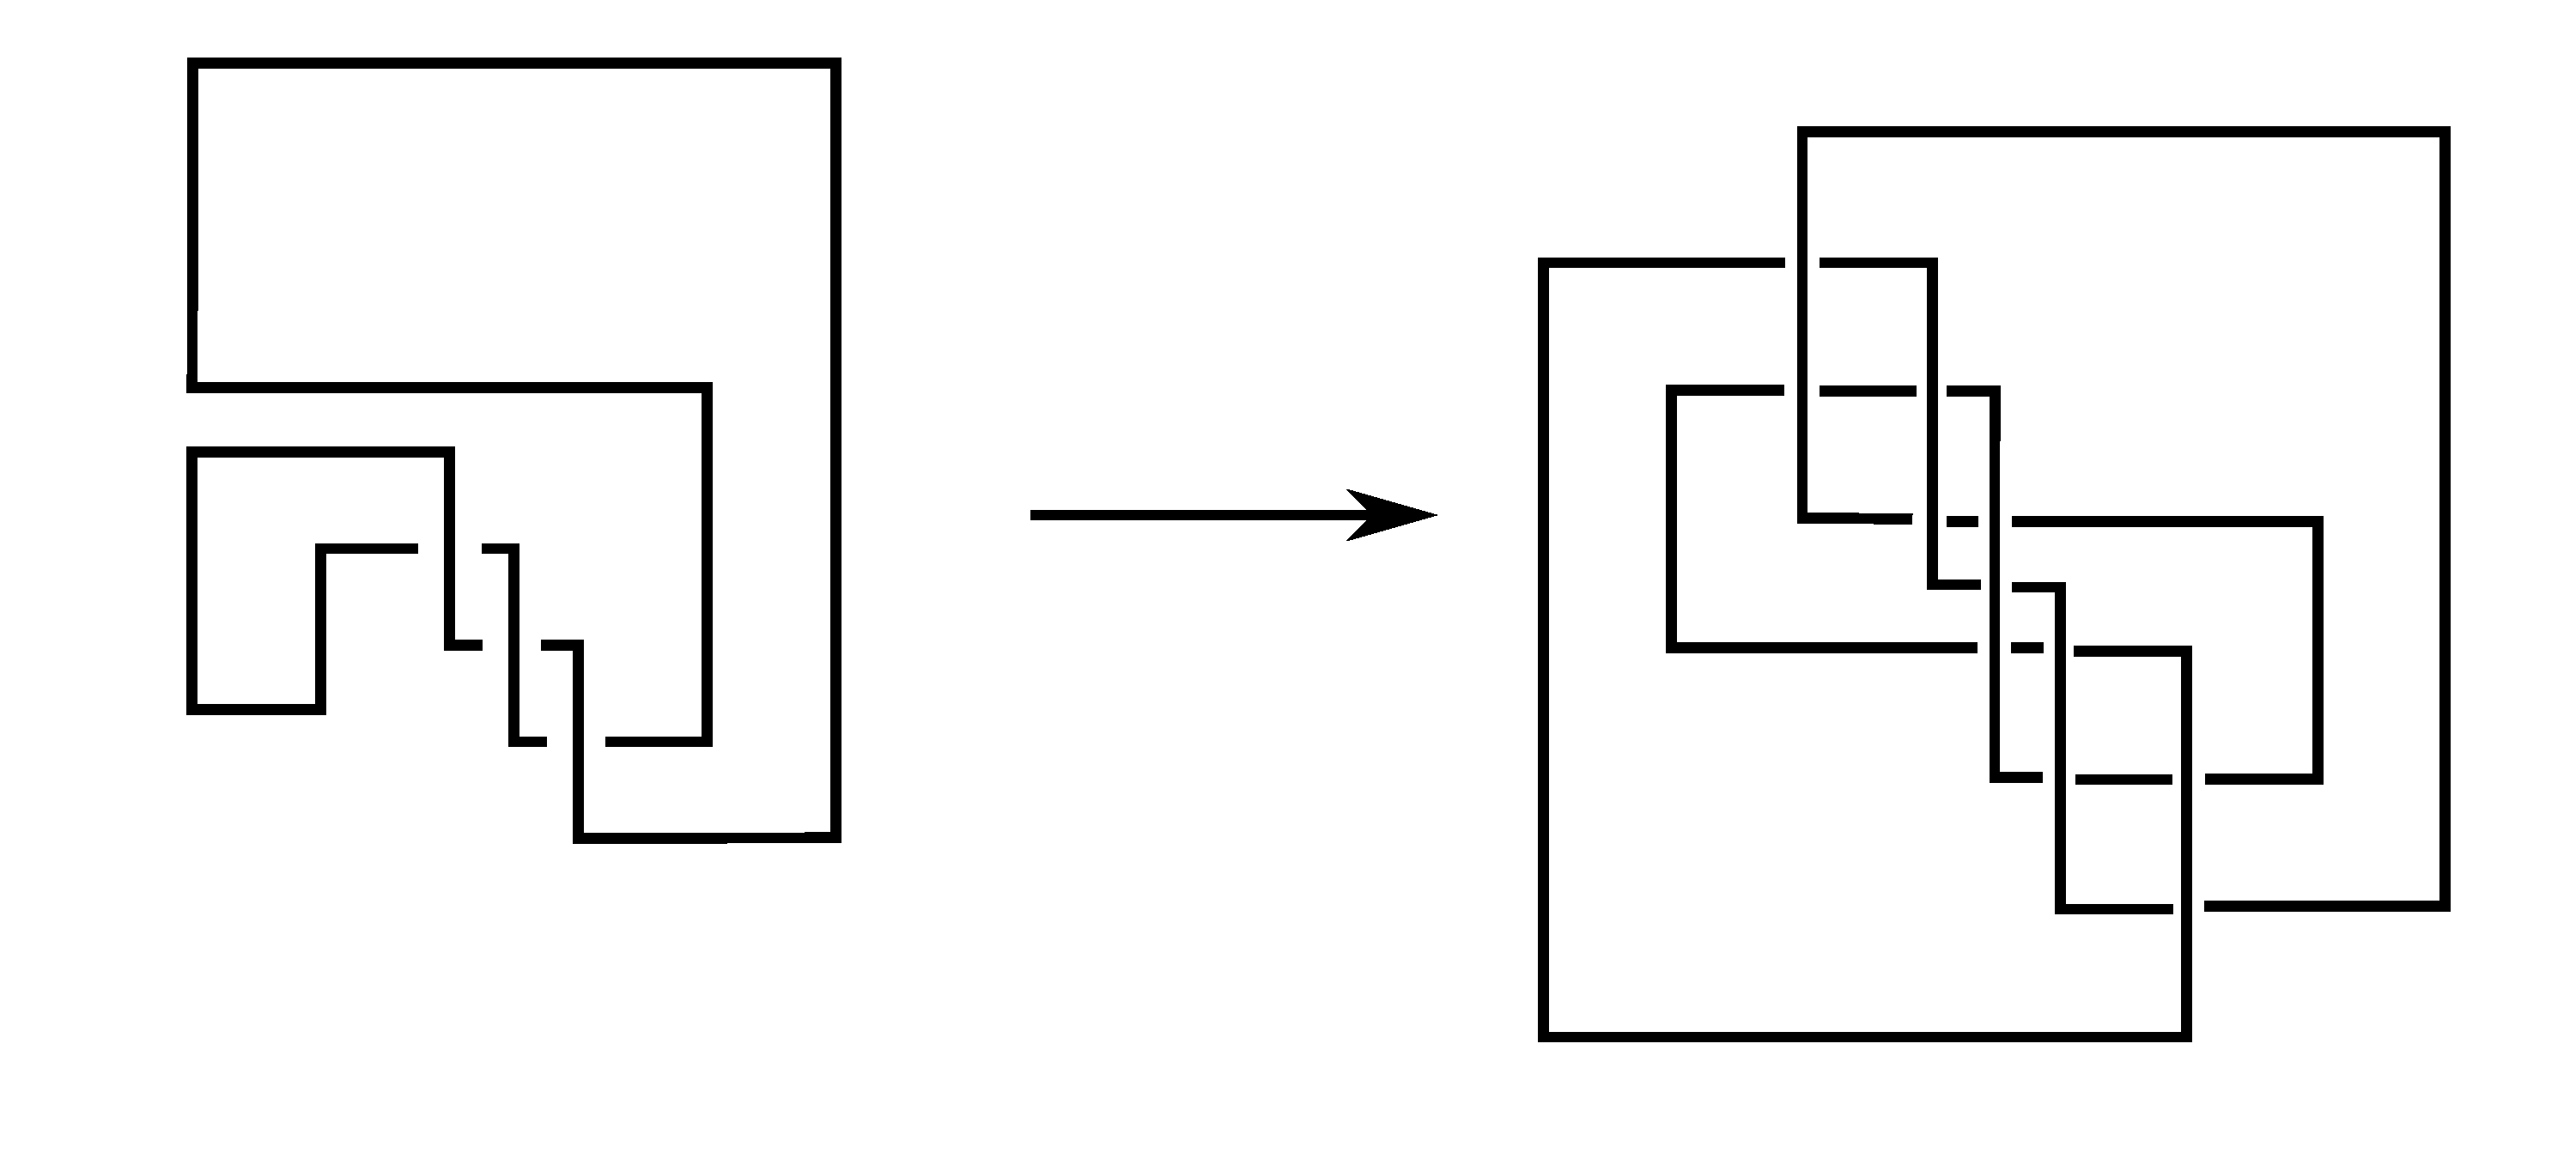
\includegraphics[width=0.4\textwidth]{images/pretzel--2-construction.pdf}
            \label{fig:pretzel-2}
            \caption{Unknot and resulting diagram for $P_{-2}$. THESE ARE LEFT TWISTS}
        \end{figure}

    \item[$1 \leq n \leq 3$ :]
        Depending on $n$ this is $6_1$, $8_{20}$, or $9_{46}$. Each has a slightly different placement of twists.
        \begin{figure}[ht!]
            \centering
            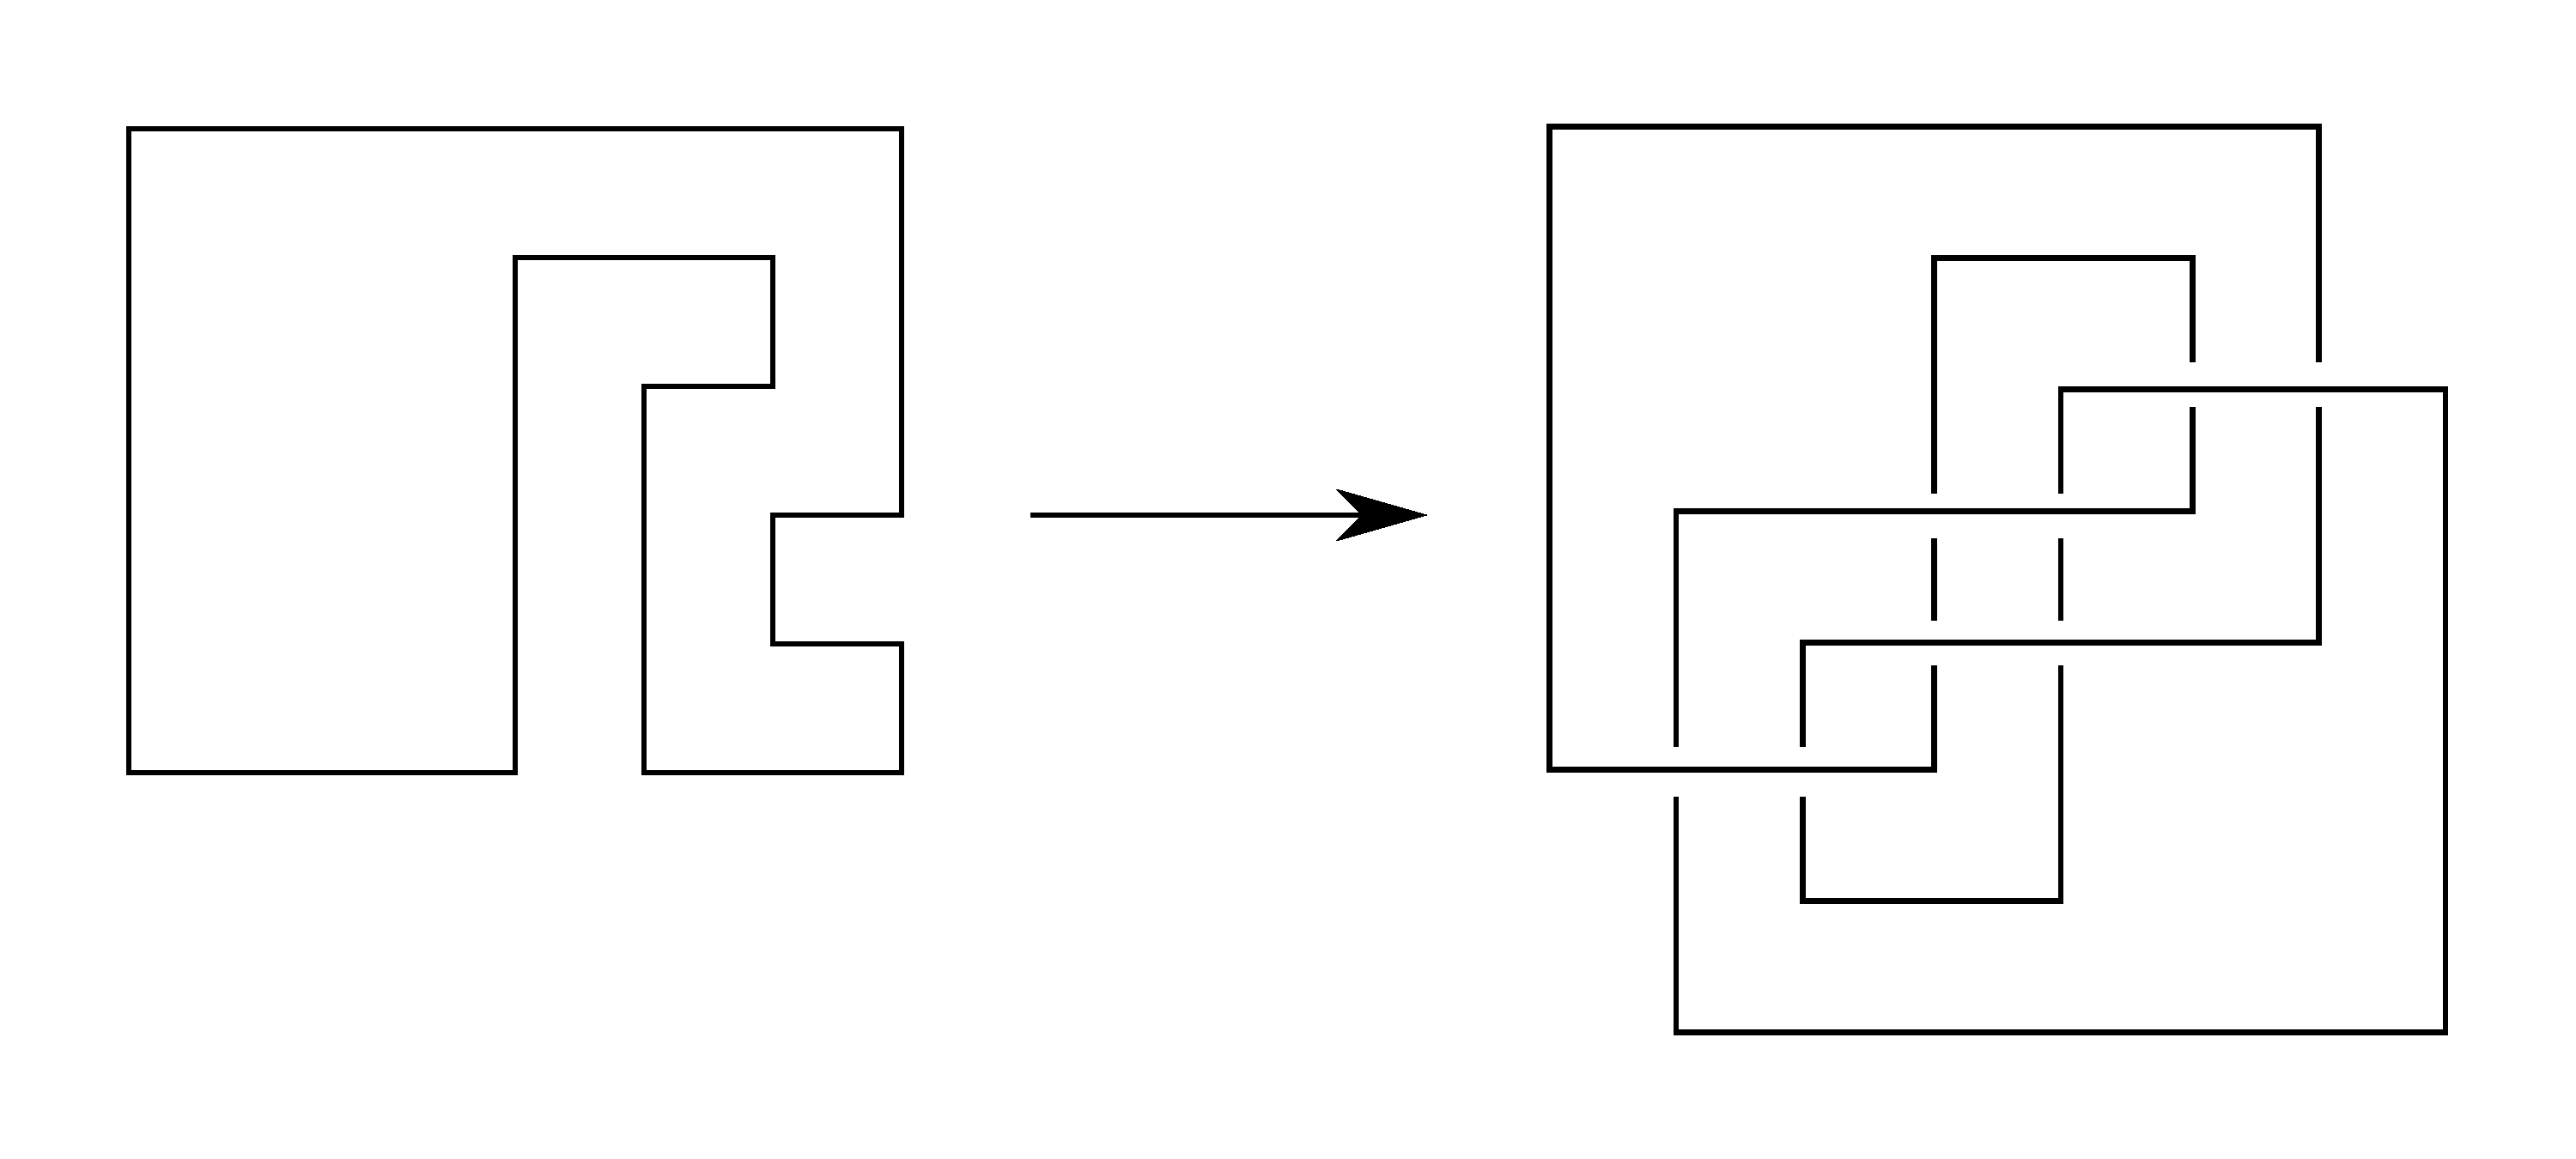
\includegraphics[width=0.3\textwidth]{images/pretzel-+1-construction.pdf} \hfill
            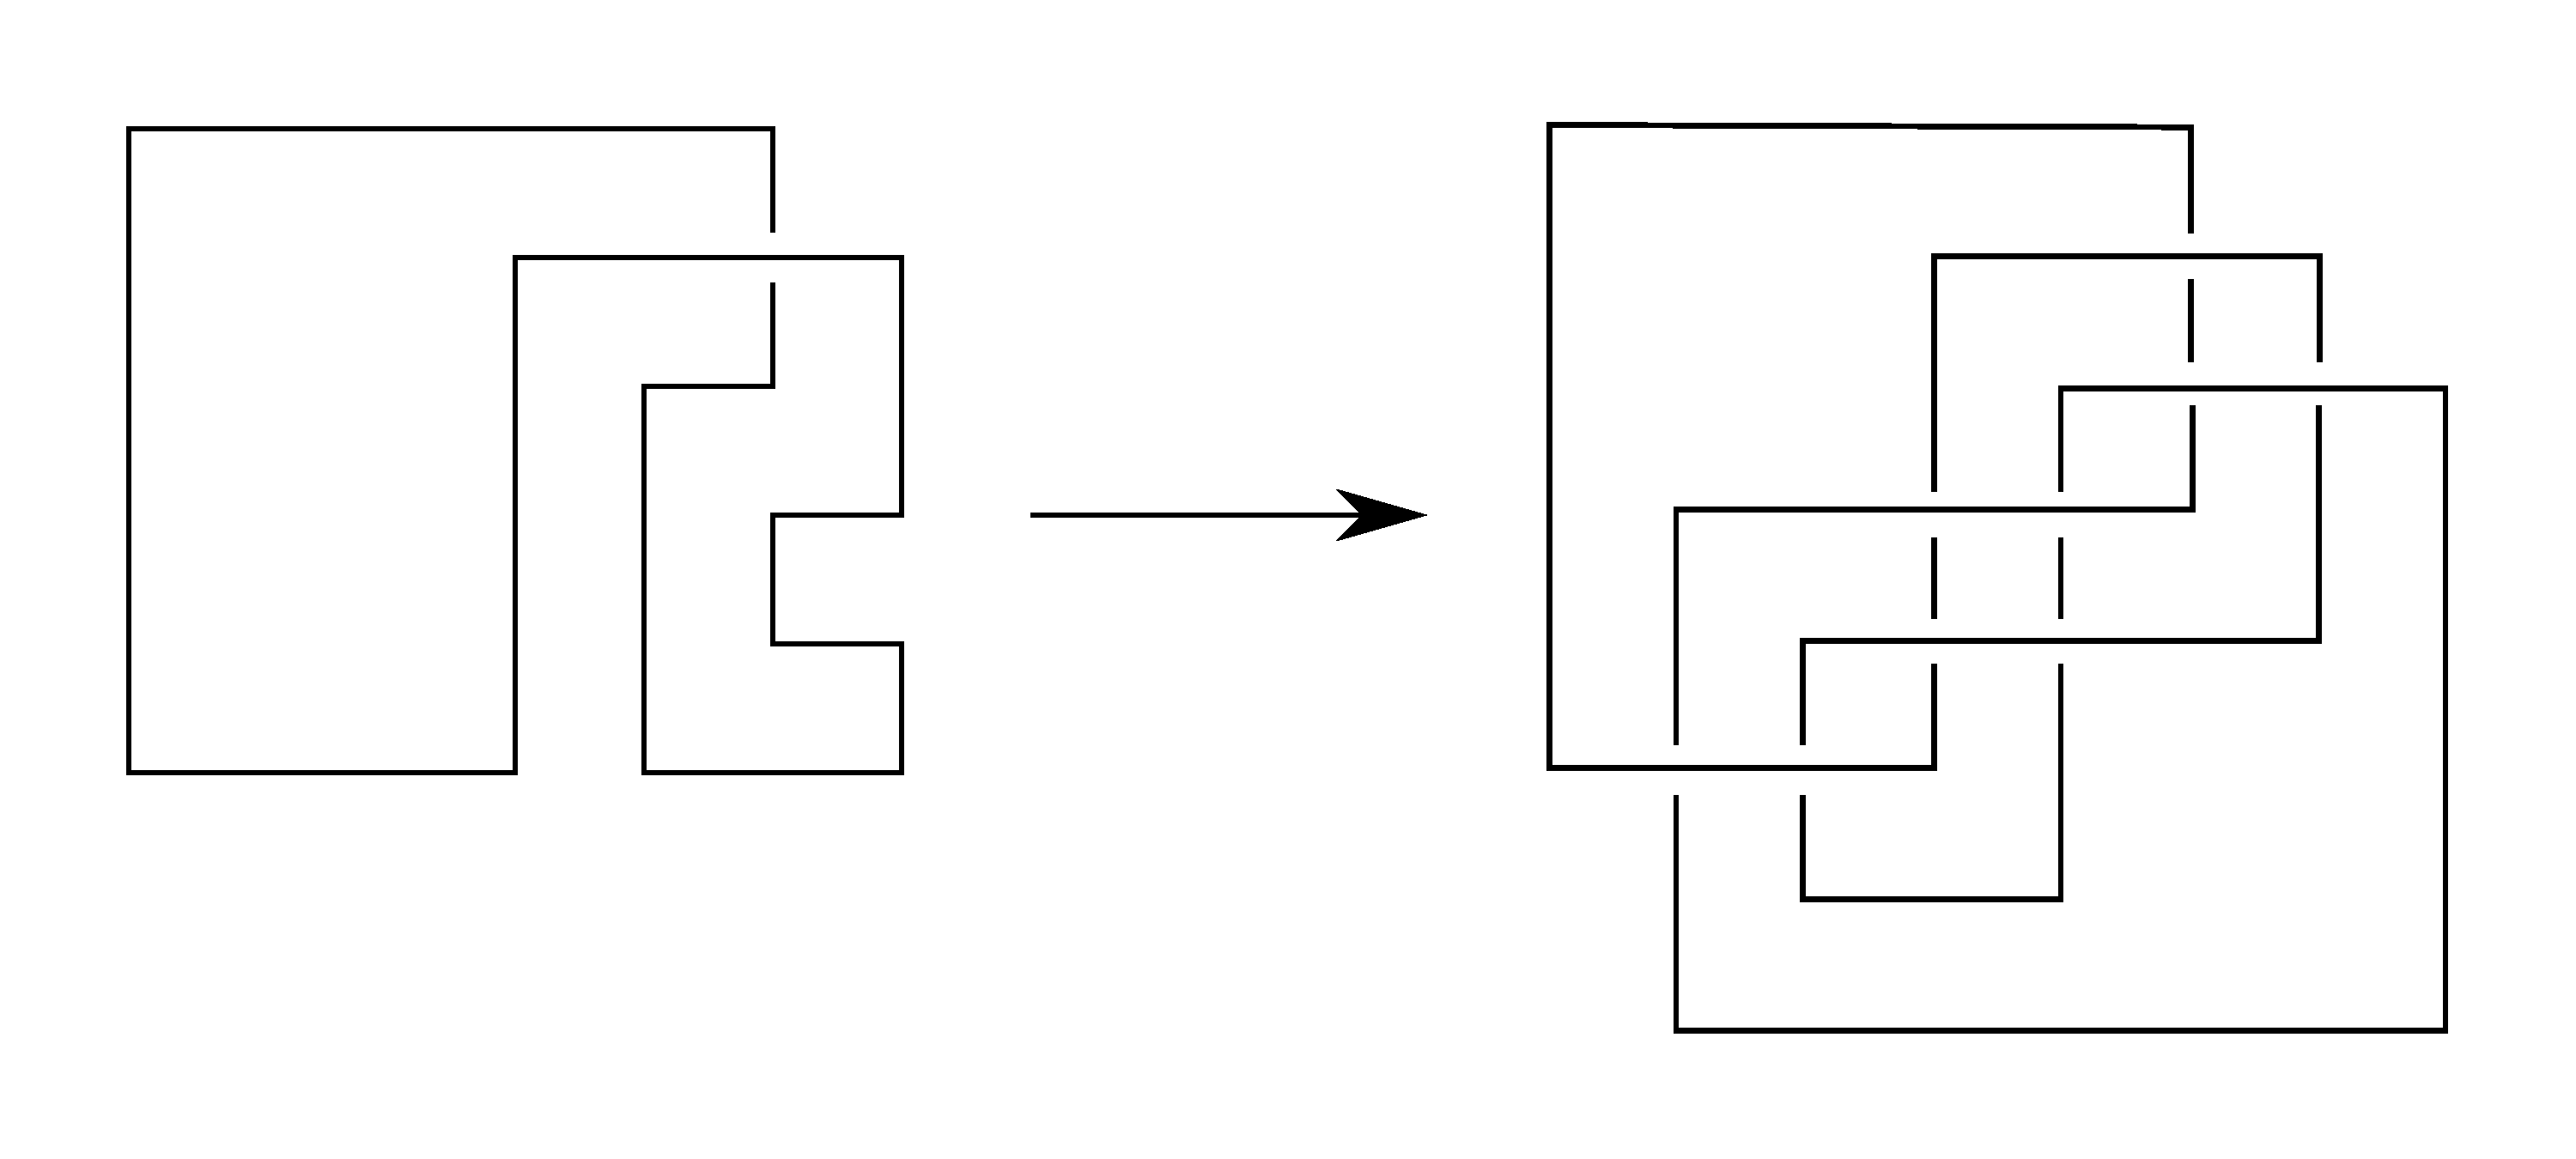
\includegraphics[width=0.3\textwidth]{images/pretzel-+2-construction.pdf} \hfill
            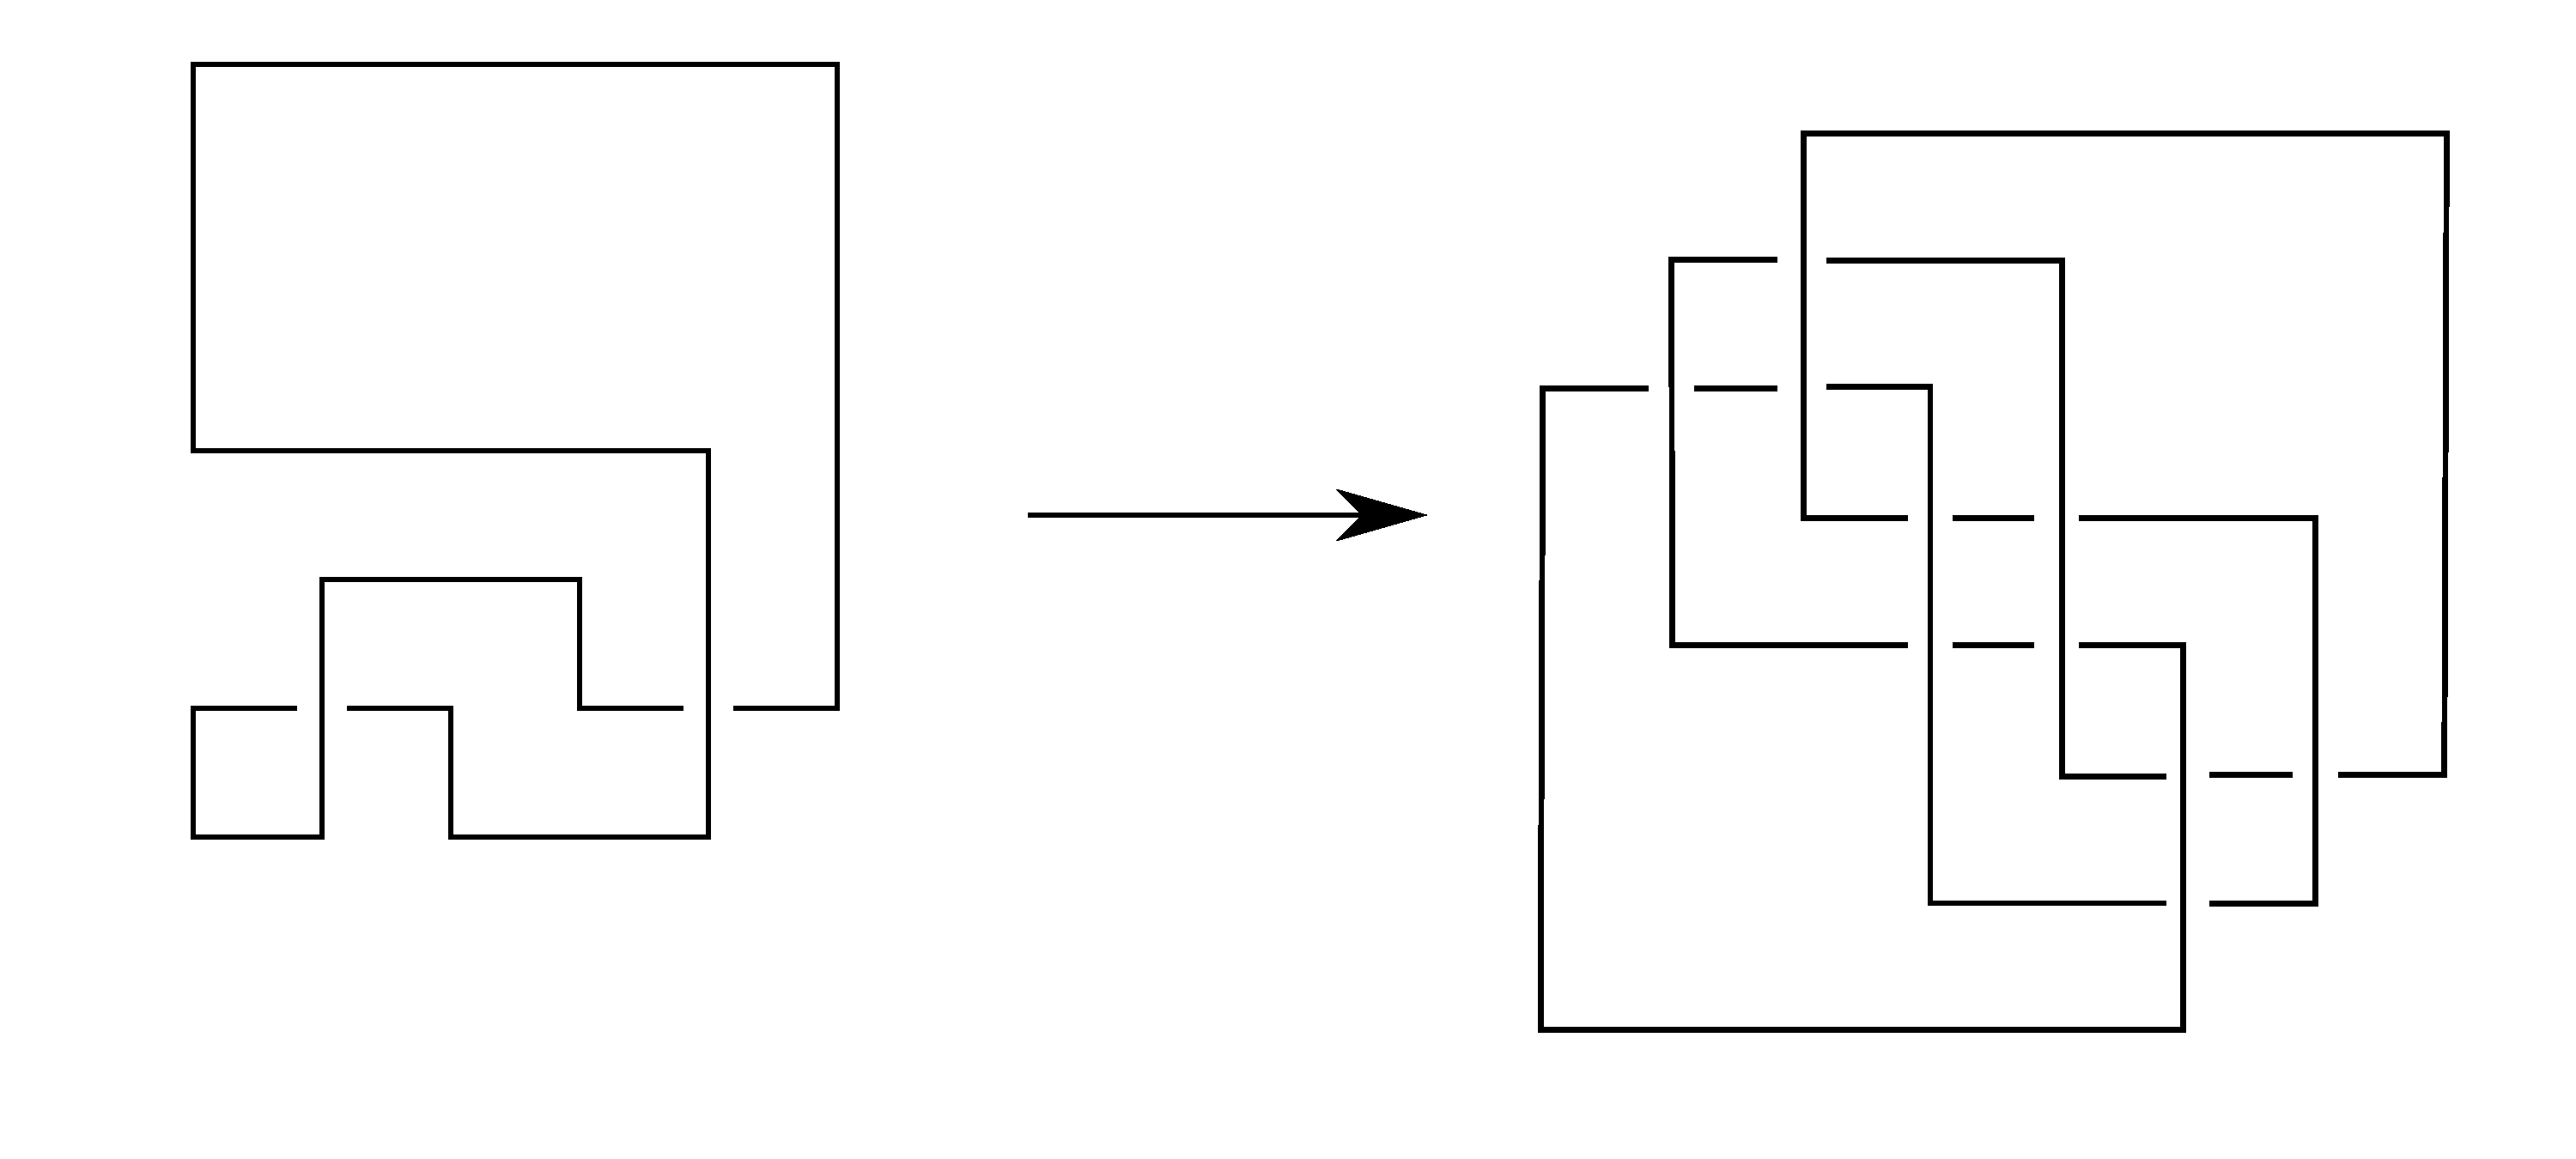
\includegraphics[width=0.3\textwidth]{images/pretzel-+3-construction.pdf}
            \label{fig:pretzel-singles}
            \caption{Unknots and resulting diagrams for $P_1$, $P_2$, and $P_3$ respectively.}
        \end{figure}

    \item[$n \geq 4$ :]
        The desired $\tb$ is $-1$. Using the RI move we can add as many right half-twists as we like (i.e., $n - 1$) to our unknot before we make the pinch move.
        \begin{figure}[h!]
            \centering
            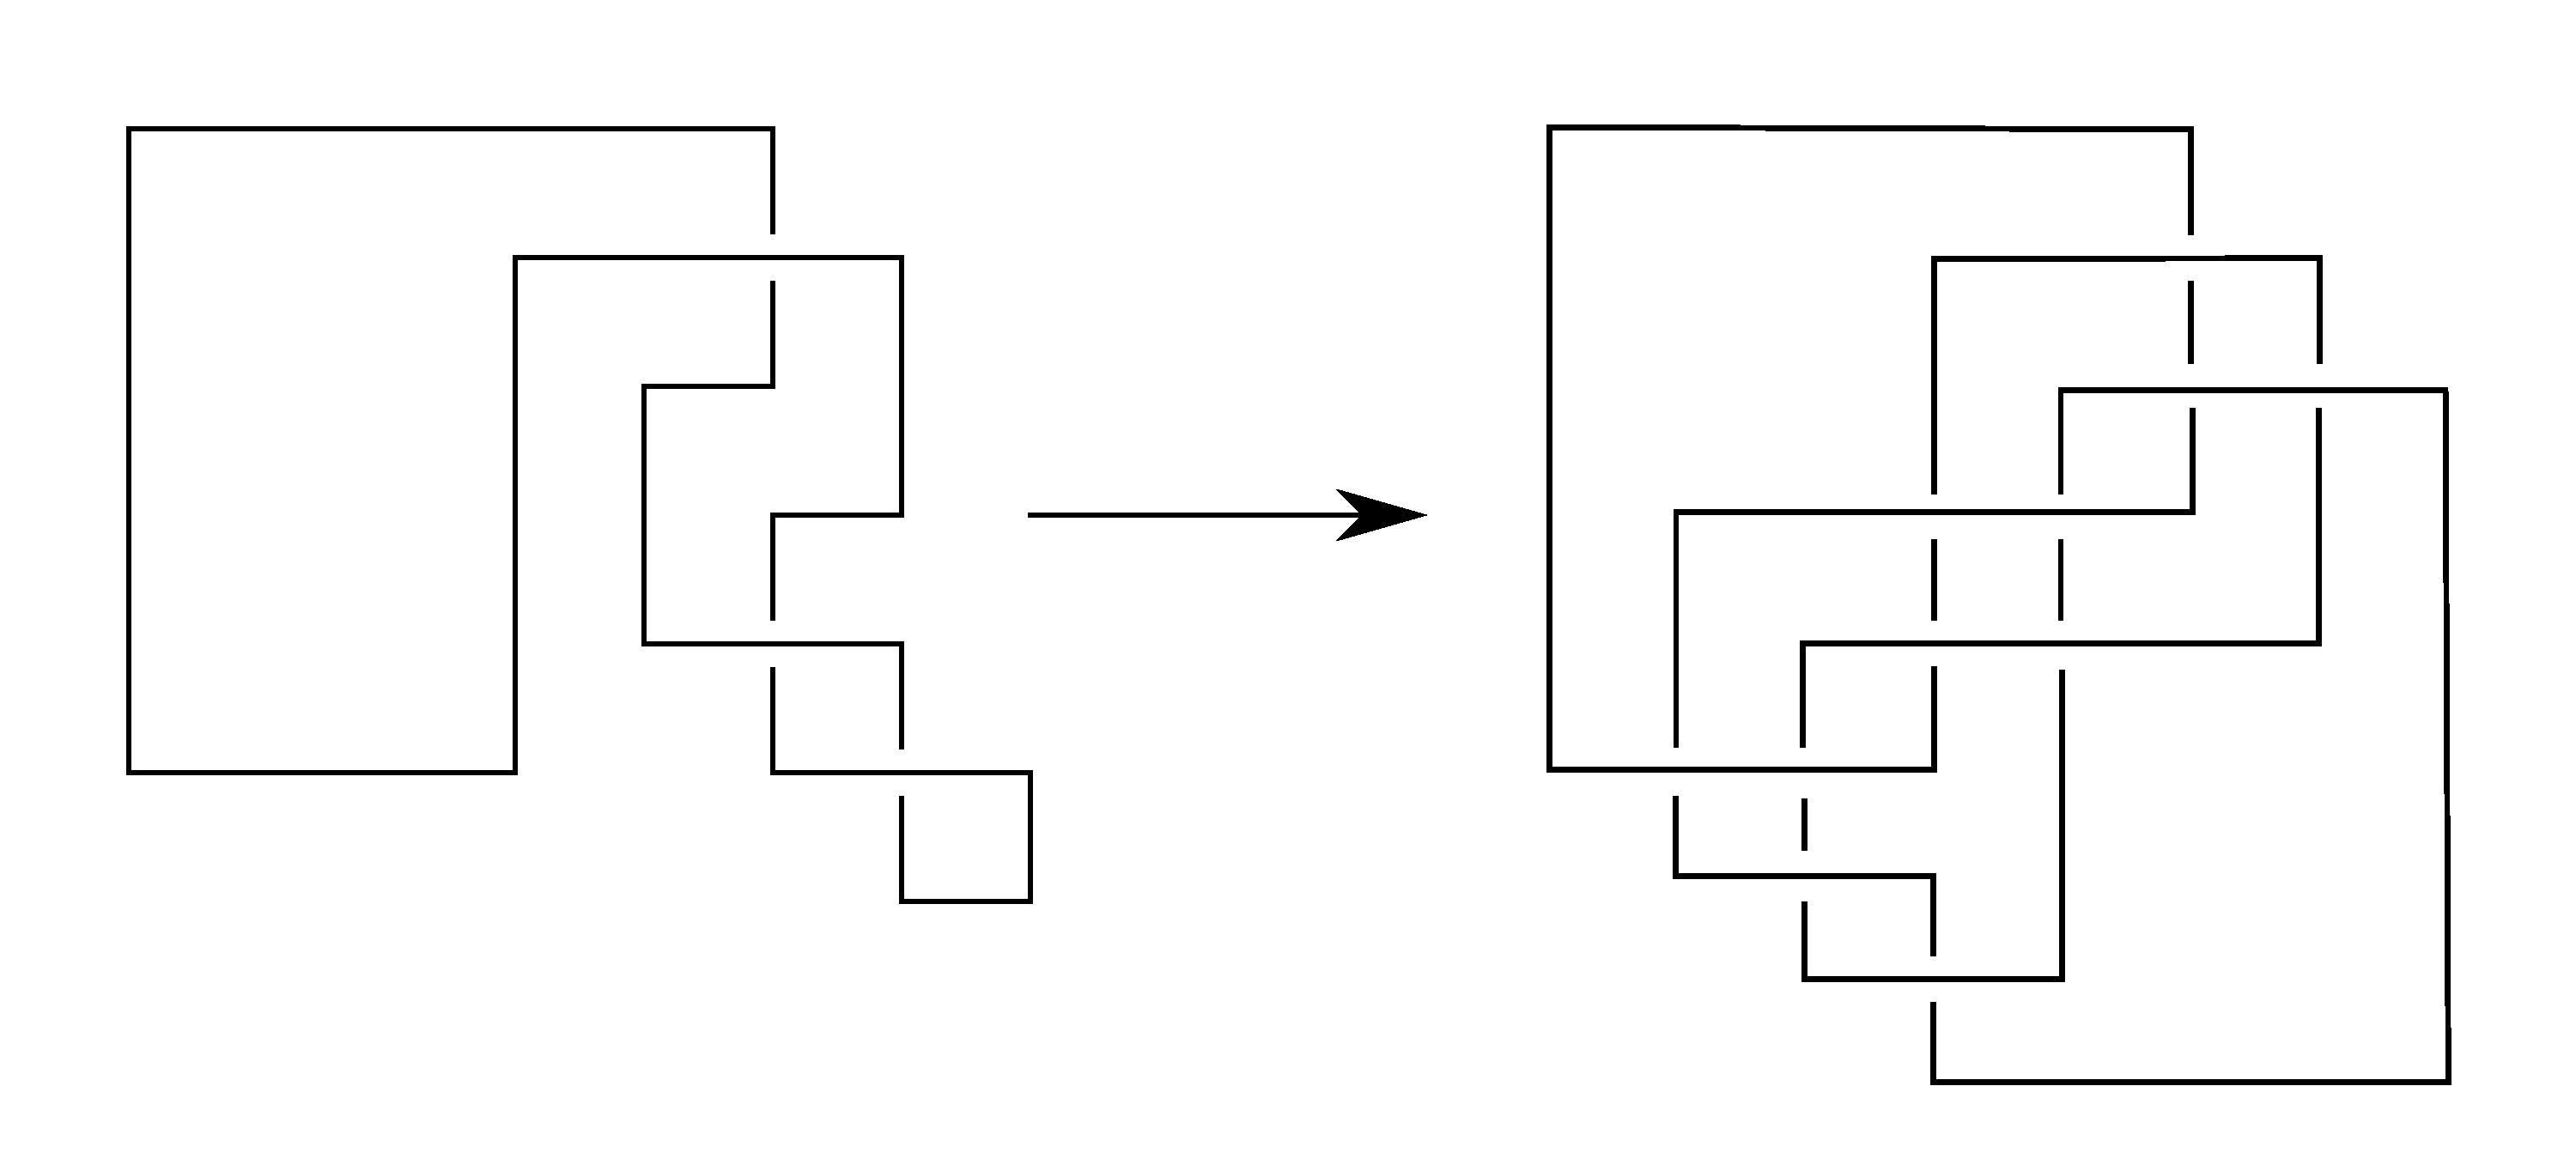
\includegraphics[width=0.4\textwidth]{images/pretzel-+4-construction.pdf}
            \label{fig:pretzel+4}
            \caption{Unknot and resulting diagram for $P_{4}$.}
        \end{figure}

\end{itemize}

\end{proof}
